\documentclass[sommairechap,stylebook]{clsbook}

\newcommand\red[1]{{\color{red}#1}}
\newcommand\blue[1]{{\color{blue}#1}}

\definecolor{mygreen}{rgb}{0,0.6,0}
\definecolor{mygray}{rgb}{0.5,0.5,0.5}
\definecolor{mymauve}{rgb}{0.58,0,0.82}

\lstset{ %
  backgroundcolor=\color{white},   % choose the background color; you must add \usepackage{color} or \usepackage{xcolor}; should come as last argument
  basicstyle=\footnotesize,        % the size of the fonts that are used for the code
  breakatwhitespace=false,         % sets if automatic breaks should only happen at whitespace
  breaklines=true,                 % sets automatic line breaking
  captionpos=b,                    % sets the caption-position to bottom
  commentstyle=\color{mygreen},    % comment style
  deletekeywords={...},            % if you want to delete keywords from the given language
  escapeinside={\%*}{*)},          % if you want to add LaTeX within your code
  extendedchars=true,              % lets you use non-ASCII characters; for 8-bits encodings only, does not work with UTF-8
  frame=single,	                   % adds a frame around the code
  keepspaces=true,                 % keeps spaces in text, useful for keeping indentation of code (possibly needs columns=flexible)
  keywordstyle=\color{blue},       % keyword style
  language=Octave,                 % the language of the code
  morekeywords={*,...},           % if you want to add more keywords to the set
  numbers=left,                    % where to put the line-numbers; possible values are (none, left, right)
  numbersep=5pt,                   % how far the line-numbers are from the code
  numberstyle=\tiny\color{mygray}, % the style that is used for the line-numbers
  rulecolor=\color{black},         % if not set, the frame-color may be changed on line-breaks within not-black text (e.g. comments (green here))
  showspaces=false,                % show spaces everywhere adding particular underscores; it overrides 'showstringspaces'
  showstringspaces=false,          % underline spaces within strings only
  showtabs=false,                  % show tabs within strings adding particular underscores
  stepnumber=2,                    % the step between two line-numbers. If it's 1, each line will be numbered
  stringstyle=\color{mymauve},     % string literal style
  tabsize=2,	                   % sets default tabsize to 2 spaces
  title=\lstname                   % show the filename of files included with \lstinputlisting; also try caption instead of title
}

\begin{document}
 
% ==================================================================
% OPTIONS D'AFFICHAGE
% non-d�finitif (soumis aux rapporteurs) ou  d�finitif
\definitiftrue
% \definitiffalse
 
% ==================================================================
% RENSEIGNEMENTS SUR LE DOCUMENT
 
\titleFR{'smartplus' documentation}
\titleEN{'smartplus' documentation}
\abstractFR{Le r�sum� en fran�ais ($\approx$ 1000 caract�res)}
\abstractEN{Le r�sum� en anglais ($\approx$ 1000 caract�res)}
\keywordsFR{Simulation num�rique}
\keywordsEN{Numerical simulation}
 
\author{smartplus team}
\address{yves.chemisky@ensam.eu}
\universite{Arts et M�tiers Metz, TU Bergakademie Freiberg}
%\laboratoire{LEM3}

% DEBUT DE LA PREFACE
\beforepreface

% remerciements
%\include{remerc}
 
% table des mati�res g�n�rale
\tableofcontents

%\cleardoublepage
% affiche la liste des figures
%\listoffigures
%\cleardoublepage
% affiche la liste des tables 
%\listoftables
\cleardoublepage

% ==================================================================
\afterpreface
 
% ==================================================================
% AVANT-PROPOS
%\include{intro}
\adjustmtc
 
% ==================================================================
% CONTENU G�N�RAL
\part{Practical documentation}
\chapter{Identification of material parameters}
\label{chap:constitutive_models}

\resumechap{}

\hphantom{a}

With the design of new devices with complex geometry and to take the most advantage of the materials utilized, the local loading paths are often strongly multiaxial while the material often operates a non-linear regime. The development of new structures requires the prediction of their thermomechanical response, for which the calibration of the material parameters for the numerical model is an important step. For other applications, the identification of parameters characteristics of the microstructure (e.g. orientation density function of fiber reinforcements) is crucial to be able to properly describe the effective response of a composite material at a global scale level.

A robust, versatile parameter identification method is thus required. In most cases, the parameter identification do not resume to only find an optimization algorithm that will be able to minimize a given function. An integrated approach that controls all the workflow of the parameter identification procedure is required, with the definition of the function to minimize , the additional constraints and set up the model that will compute the trial numerical values to be compared with experimental data. A typical view of 

Various optimization algorithms have been used in identification methods, i.e. deterministic algorithms such as gradient-based Levenberg-Marquardt algorithm~\citep{Levenberg.1944, Marquardt.1963}, real space evolutionary-inspired, genetic algorithms or Bayesian statistical approaches~\citep{Beck&Arnold.1977}. The Levenberg-Marquardt optimization algorithm has been often adopted for the determination of material parameters for metals~\citep{Springmann&Kuna.2005, Mahnken&Stein.1996, Ghouati&Gelin.1998, Cooreman.etal.2007}. 
An hybrid algorithm that used an evolutionary algorithm combined with a gradient-based algorithm has been utilized by \cite{Chaparro.etal.2008} to determine the parameters of an elastic-plastic constitutive model including an anisotropic criterion~\citep{Barlat.etal.1991} coupled with a non-linear kinematical hardening \citep{Lemaitre&Chaboche.1990}. The evolutionary algorithm was used to determine a good initial guess values for the gradient-based approach and therefore ensure that a local minima has been found.

\begin{figure}
\begin{center}
 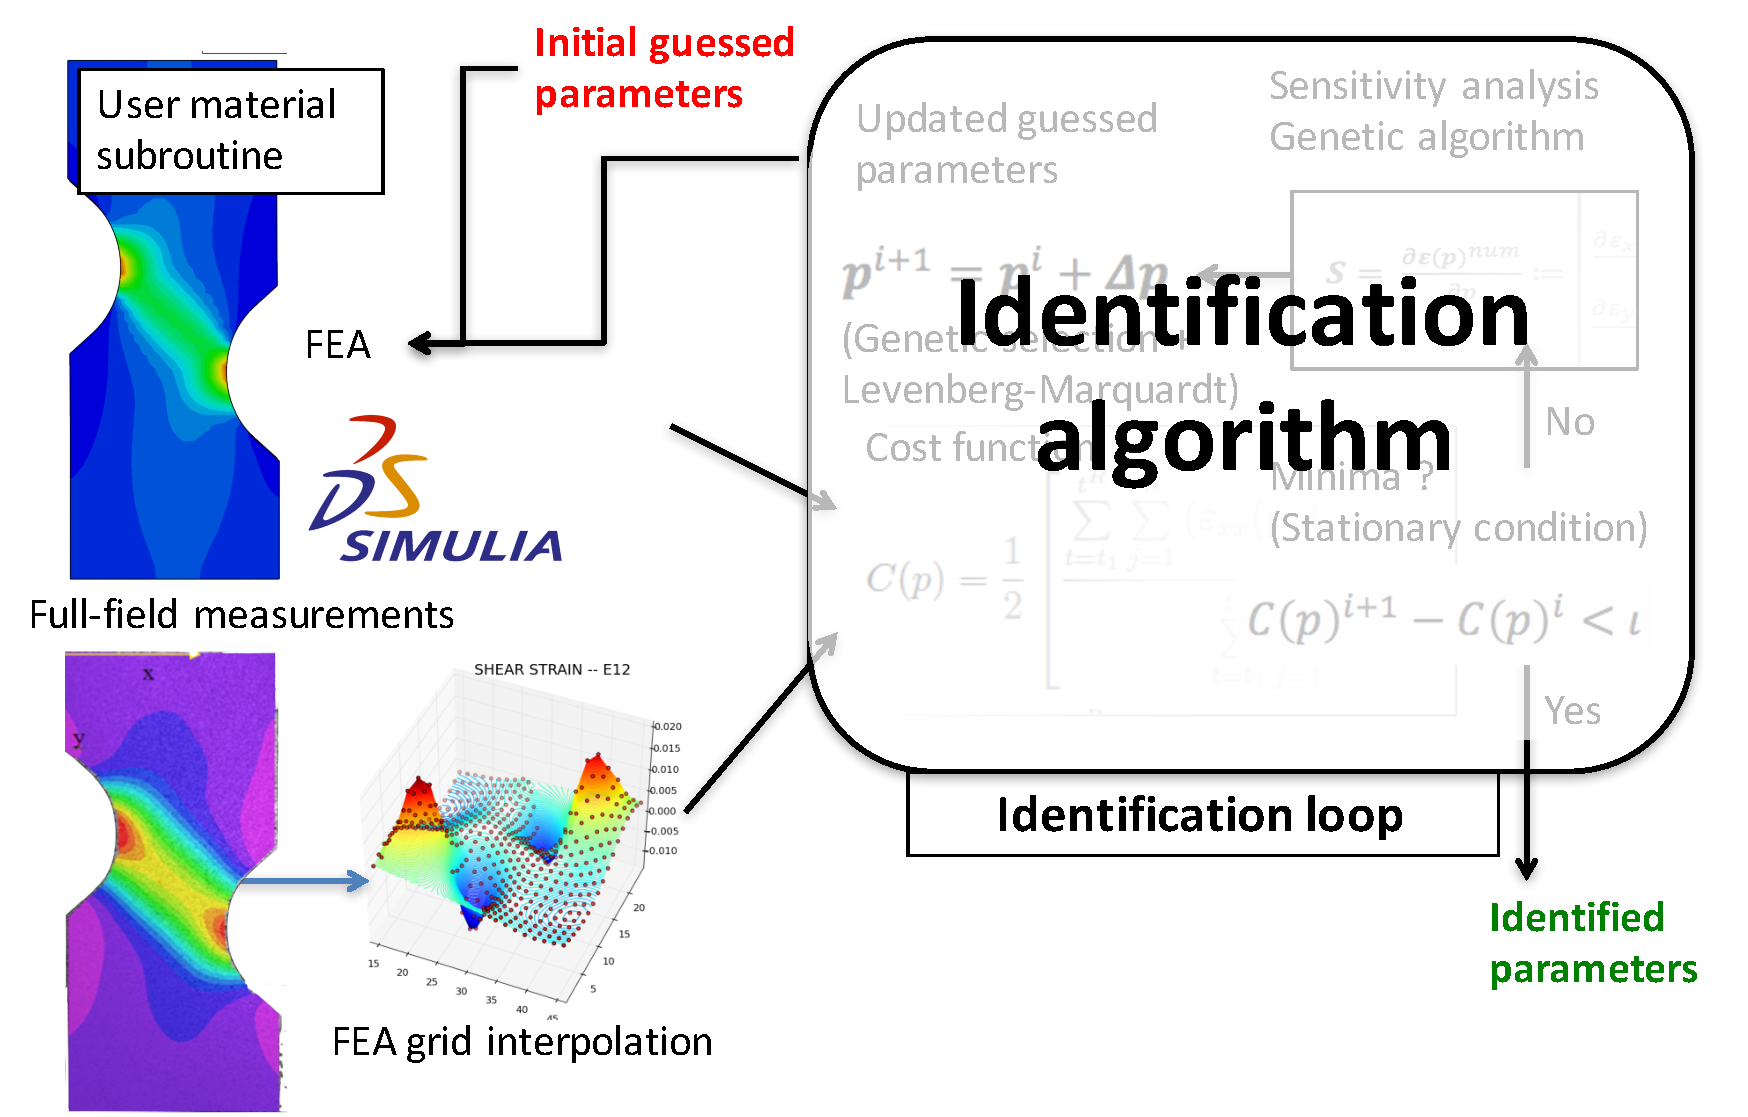
\includegraphics[width=0.8\textwidth]{1_Identification/identification-procedure}
 \caption{Overview of the identification procedure}
 \label{fig:identproc}
\end{center}
\end{figure}

In this chapter, the parameters of a phenomenological model are extracted from tests performed on specimens with non-uniform geometry, which induce heterogeneous strain fields carried out on specimens with the same thermomechanical loading history. The digital image correlation technique is employed to measure the strain fields on the surface of the specimen and to analyze the strain paths of chosen points. Finite element analysis enables the computation of numerical strain fields using a thermodynamical constitutive model for shape memory alloys previously implemented in a finite element code. The strain fields computed numerically are compared with experimental ones obtained by DIC to find the model parameters which best match experimental measurements using a newly developed parallelized mixed genetic/gradient-based optimization algorithm.  These numerical simulations are carried out in parallel using a supercomputer to reduce the time necessary to identify the set of model parameters. The major features of this new algorithm is its ability to identify the material parameters which describe the thermomechanical behavior of shape memory alloys from full-field measurements for various loading conditions (different temperatures, multiaxial behavior, heterogeneous test configurations).
It is demonstrated that model parameters for the simulation of SMA structures are thus obtained based on a reduced number of heterogeneous tests at different temperatures.

\section{Description of the workflow}
\label{sec:workflow}

\subsection{Definition of the objective function}

Having any type of numerical model with specific set of material parameters, the identification problem consists in the determination of a prescribed set of material parameters that minimize the difference between computed data and a set of experimental data. The numerical model could be typically a Finite Element model, with the same geometry and boundary conditions than the experimental setup. A part of the experimental results is in this case utilized to define (or to complete the definition) of the boundary value problem to solve using the finite element method and another part is utilized to define a cost function to be minimized.

A general cost function is considered to be:

\begin{equation}
C(\mathbf{p}) = \frac{1}{2} \sum_i w_i \left( {v_i^{num}(\mathbf{p}) - v_i^{exp}} \right)^2
\end{equation}

\noindent where $C(\mathbf{p})$ is the cost function, $v_i^{num}(\mathbf{p})$ is the i-th information obtained with the numerical simulation, $v_i^{exp}$ is the i-th information obtained from the set of experiments conducted and $w_i$ is a weight factor. Note that all these information are potentially obtained from a number of experiments at different times and at different spatial positions.

In the methodology proposed here, the experimental data are classified in the following:

\begin{itemize}
\item Each experiment is considered separately and is determined with the index $e$
\item Within that experiment, there exists a number $n$ of measured quantities
\item Within an experiment, there exist a number $j$ of experimental points
\end{itemize}

The cost function is therefore set as: 

\begin{equation}
C(\mathbf{p}) = \frac{1}{2} \sum_e \sum_n \sum_j w_e w_{e,n} w_{e,j,n} \left( {v_{e,j,n}^{num}(\mathbf{p}) - v_{e,j,n}^{exp}} \right)^2,
\end{equation}

\noindent where the three weights factors $w_{e}$, $w_{e,n}$ $w_{e,n,j}$ can be set independently.

\subsubsection{Information about the experimental points}

The information about the experimental points to be compared with have to be set in the file "files\_exp.inp". The file that correspond to the example described here is presented below:

\lstinputlisting[language=Verilog, frame=single]{1_Identification/files_exp.inp}

The first part "\#Name\_of\_the\_exp\_files" is directly followed with the name of the files that are stored in the~\emph{exp\_data} folder. The number of files should correspond to what indicated in the file "data\/ident\_essentials.inp" and correspond to the \{e\} index:
\begin{itemize}
\item results\_0-90.dat
\item results\_pm45.dat
\item results\_pm675.dat
\end{itemize}

The second part "\#EXP\_Nb\_columns\_in\_files" is directly followed with the number of columns of the experimental files\footnote{this will be suppressed and automatically evaluated in a subsequent version}:
\begin{itemize}
\item 20
\item 20
\item 20
\end{itemize}

The three file then are composed of 20 columns.

The third part "\#EXP\_Nb\_columns\_to\_identify" is directly followed with the number of columns. It directly correspond to the \{n\} index.
\begin{itemize}
\item 2
\item 2
\item 2
\end{itemize}

The fourth part "\#EXP\_colums\_to\_identify" is directly followed with the index of the columns that contains experimental values for each experimental point. Each column correspond to the \{j\} index.

\begin{itemize}
\item $8 \quad 9$
\item $8 \quad 9$
\item $8 \quad 9$
\end{itemize}

The fifth and last part  "\#skip\_lines" corresponds to the number of lines that are skipped and usually correspond to a header in the files.

\begin{itemize}
\item $0$
\item $0$
\item $0$
\end{itemize}

\subsubsection{Information about the weight factors}

In the file "files\_weights.inp", you can enter those weight factors in the following manner:

\lstinputlisting[language=Verilog, frame=single]{1_Identification/files_weights.inp}

The final version of the cost function is written as:


\begin{equation}
\begin{split}
C(\mathbf{p}) & = \frac{1}{2} \alpha_{\varepsilon} \left( \frac{ \sum_i \sum_t \sum_T \left( \varepsilon_{xx}^{num}(\mathbf{p}) - \varepsilon_{xx}^{exp} \right)^2 }{ \sum_i \sum_t \sum_T \left( \varepsilon_{xx}^{exp} \right)^2 } 
 +  \frac{ \sum_i \sum_t \sum_T \left( \varepsilon_{yy}^{num}(\mathbf{p}) - \varepsilon_{yy}^{exp} \right)^2 }{ \sum_i \sum_t \sum_T \left( \varepsilon_{yy}^{exp} \right)^2 } \right. \\
& + \left.  \frac{ \sum_i \sum_t \sum_T \left( \varepsilon_{xy}^{num}(\mathbf{p}) - \varepsilon_{xy}^{exp} \right)^2 }{ \sum_i \sum_t \sum_T \left( \varepsilon_{xy}^{exp} \right)^2 } \right)
 + \frac{1}{2} \alpha_{F} \left( \frac{ \sum_i \sum_t \left( F^{num}(\mathbf{p}) - F^{exp} \right)^2 }{ \sum_i \sum_t \left( F^{exp} \right)^2 } \right)
\end{split}
\end{equation}

\noindent where $\varepsilon^{exp}_{xx}$, $\varepsilon^{exp}_{yy}$ and $\varepsilon^{exp}_{xy}$ represent the three components of  the strain tensor that are extracted at a material point $i$ of coordinates $\b{x}_i$ at the time $t$ from an isothermal test performed at the temperature $T$. The values $\varepsilon^{num}_{xx}$, $\varepsilon^{num}_{yy}$ and $\varepsilon^{num}_{xy}$ represent the corresponding values computed using a chosen constitutive model. $p$ denotes the set of guessed parameters. The weight parameters $\alpha_{\varepsilon}$ and $\alpha_{F}$ are set to equilibrate the influence of the error in strains and the error in reaction force. The total contribution to the cost function of the strain and the force has been set to be about half for each component, which is obtained using $\alpha_{\varepsilon} = 1$ and $\alpha_{F} = 40$.

\subsection{Optimization algorithm}
\label{sec:defalgo}

The definition of an optimization algorithm has to take into account the computational time necessary to perform a numerical simulation for a given set of parameters. Indeed, it often depends on the model utilized to obtain values entering in the definition of the cost function according to a given set of design variables. Especially, the efficiency of the algorithms depends on the time necessary to compute a numerical solution and then evaluate the corresponding cost to be able to evaluate the prescribed set of parameters within the set of admissible solutions. Also, the form of the cost function might impact the decision of an optimization algorithm, e.g. if local minima are expected.
Indeed, the main issue associated with gradient-based techniques is that the method ensures the convergence to a {\it local} minima. Heuristic such as genetic algorithm should be therefore utilized in such cases to determine preferential sets of parameters from a large population that are close to the global minima~\citep{Chaparro.etal.2008}.
In the approach proposed, the genetic algorithm and the gradient-based method are used simultaneously, with the following procedure:

\begin{enumerate}
\item An initial population of $C_0$ individuals (each individual is a set of parameters) is generated. The selection of individuals can be aleatory, given limitations of the material parameters, or can be generated using Design Of Experiments (DOE).
\item The numerical simulation for all the individual is computed {\it in parallel}.
\item All the individuals are scored by computing their cost value.
\item The individuals of the initial generation are classified, and a number $n$ of them are selected (the best ones). These constitute the 'current' generation $n$.
\item	A set of children of the current generation (with $n$ members) are determined using the crossover technique. A mutation probability has been added to increase the diversity of the children generation. For the same purpose a small deviation operator from the parent's parameters is also applied.
\item The bests members of the current generation are selected. The set of numerical simulation to apply the finite differences derivation technique is determined.
\item The numerical simulation for all the children and the simulations required for the finite differences derivation are computed {\it in parallel}.
\item The cost function of all the individual is determined.
\item The parameters of a number $N_{GB}$ of the best members are updated using a Levenberg-Marquardt algorithm.
\item The current generation $n+1$ is determined from the the best individuals among the current generation $n$ and the children.
\item Stationary condition test for the best individual of the current generation compared to the previous best. If needed, reloop from item $5$.
\end{enumerate}

On overview of the identification procedure in general is presented in Figure~\ref{fig:identproc}.

\red{\subsection{Identification of the material parameters based on the heterogeneous Meuwissen experiments}}

\red{The identification method presented in section~\ref{sec:procedure} is applied to the case of a set of experimental data corresponding to three isothermal tests performed at 50$\celsius$, 60$\celsius$ and 70$\celsius$. }
Several tests have been conducted with different parameters of the hybrid genetic - gradient based algorithm, which are resumed in Tab.~\ref{tab:prefiden}. 

The different control parameters of the algorithm are:

\begin{itemize}
\item The initial number of individuals of the first generation $N_{init}$.
\item The number of sons generated and the number of retained individual for the current generation $N_{cur}$.
\item The number of best individuals selected to be optimized via the Levenberg-Marquardt gradient based algorithm $N_{GB}$.
\item The probability of mutation of the parameters, set to 5\%. This means that for each parameter of all the new individual, there is a 5\% chance that the concerned parameter is set randomly inside the design space rather than being selected from the crossover technique. This low value is generally utilized when a low population is defined to keep a certain stability of the generations, still slowly introducing new parameters to authorize the exploration of new points in the design space.
\item The first (best) half of each generation is considered for the crossover technique.
\end{itemize}

For each case the identification was stopped after a maximum of 30 generations, or after a stabilization of the cost function. The algorithm has been ran on a cluster to be able to parallelize the numerical simulations. This is achieved using a developed software coupled with TORQUE Resource Manager for the management of the simulation on the cluster. 

%%%%%%%%%%%%%%%%%%%%%%%BEGIN TABLE%%%%%%%%%%%%%%%%%%%%%%%%%%%%%%%%%%%%%%%%%%%%%%
\begin{table}[ht]
\caption{Parameters of the hybrid genetic - gradient based algorithm for the four identification tests}
\begin{center}
\label{tab:prefiden}
\begin{tabular}{c c c c} % put some space after the caption
\hline
Number & $N_{init}$ & $N_{cur}$ & $N_{GB}$ \\
1 & 50 & 10 & 1 \\
2 & 50 & 10 & 1 \\
3 & 150 & 50 & 1 \\
4 & 150 & 5 & 3 \\
\hline\end{tabular}
\end{center}
\end{table}
%%%%%%%%%%%%%%%%%%%%%%%END TABLE%%%%%%%%%%%%%%%%%%%%%%%%%%%%%%%%%%%%%%%%%%%%%%%

The set of initial parameters is bounded to define the design space (see Tab.~\ref{tab:parabounds}) : 

%%%%%%%%%%%%%%%%%%%%%%%BEGIN TABLE%%%%%%%%%%%%%%%%%%%%%%%%%%%%%%%%%%%%%%%%%%%%%%
\begin{table}[ht]
\caption{Min and max bounds for the material parameters}
\begin{center}
\label{tab:parabounds}
\begin{tabular}{c c c c c c} % put some space after the caption
\hline
$ $ &$E\,\mbox{(MPa)}$ & $\nu$ & $H_f\,\mbox{(MPa)}$ & $\varepsilon^{T}_{trac}$ \\
min & 50 000 & 0.2 & 0.5 & 0.03 \\
max & 80 000 & 0.45 & 6 & 0.05 \\
\hline
$ $ & $C^M\,\mbox{(MPa}.\celsius^{-1})$) & $C^A\,\mbox{(MPa}\celsius^{-1})$ & $M_S\,(\celsius)$ & $A_f\,\mbox{(\celsius)}$\\
min & 4 & 4 & -73 & -33 \\
max & 12 & 12 & 27 & 47 \\
\hline
\end{tabular}
\end{center}
\end{table}
%%%%%%%%%%%%%%%%%%%%%%%END TABLE%%%%%%%%%%%%%%%%%%%%%%%%%%%%%%%%%%%%%%%%%%%%%%%


\section{Description of the optimization algorithm utilized}
\label{sec:workflow}


%\setcounter{chapter}{5}
%\include{6_Martensitic_Materials}
 
% ==================================================================
% CONCLUSION
%\include{concl}
 
% ==================================================================
% ANNEXES
%\appendix
%\include{annexe}
 
% ==================================================================
% BIBLIOGRAPHIE

\bibliographystyle{plainnat1}

\bibliography{HdR}
 
% ==================================================================
% NOTATIONS
%\include{nota}
 
% ==================================================================
% COLOPHON
%\colophon{Ce document a �t� r�dig� avec de l'environnement de composition typographique \LaTeXe.}
 
% ==================================================================
% COUVERTURE : RESUME ET MOTS-CLES
%\abstractpage
 
\end{document}
